%-----------------------------------------------------------------
%	BASIC DOCUMENT LAYOUT
%-----------------------------------------------------------------
\documentclass[paper=a4, fontsize=12pt, twoside=semi, abstracton, listof=totoc, toc=left]{scrartcl}
\usepackage[T1]{fontenc}
\usepackage[utf8]{inputenc}
\usepackage{lmodern}
\usepackage{slantsc}
\usepackage{microtype}
\usepackage[british]{babel}
% \usepackage[backend=bibtex, style=phys, sorting=none, citestyle=authoryear, maxbibnames=3, maxcitenames=2]{biblatex}
\usepackage[backend=bibtex, style=trad-abbrv, sorting=none, maxbibnames=3, maxcitenames=2]{biblatex}
\addbibresource{OpenData.bib}
\makeatletter
	\def\blx@maxline{77}
\makeatother

% Sectioning layout
\addtokomafont{sectioning}{\normalfont\scshape}
\usepackage{tocstyle}
\usetocstyle{standard}
\renewcommand*\descriptionlabel[1]{\hspace\labelsep\normalfont\bfseries{#1}}
\usepackage[titletoc]{appendix}

% Empty pages
\usepackage{etoolbox}
% \pretocmd{\toc}{\cleardoubleevenemptypage}{}{}
% \pretocmd{\section}{\cleardoubleevenemptypage}{}{}
\pretocmd{\part}{\cleardoubleevenemptypage\thispagestyle{empty}}{}{}
\renewcommand\partheadstartvskip{\clearpage\null\vfil}
\renewcommand\partheadmidvskip{\par\nobreak\vskip 20pt\thispagestyle{empty}}

% Paragraph indentation behaviour
\setlength{\parindent}{0pt}
\setlength{\parskip}{0.3\baselineskip plus2pt minus2pt}
\newcommand{\sk}{\medskip\noindent}

% Fancy header and footer
\usepackage{fancyhdr}
\pagestyle{fancyplain}
\fancyhead[LO]{\thepage}
\fancyhead[CO]{}
\fancyhead[RO]{\nouppercase{\mytitle}}
\fancyhead[LE]{\nouppercase{\rightmark}}
% \fancyhead[LE]{\nouppercase{\leftmark}}
\fancyhead[CE]{}
\fancyhead[RE]{\thepage}
\fancyfoot{}
\renewcommand{\headrulewidth}{0.3pt}
\renewcommand{\footrulewidth}{0pt}
\setlength{\headheight}{13.6pt}

%-----------------------------------------------------------------
%	MATHS AND SCIENCE
%-----------------------------------------------------------------
\usepackage{amsmath,amsfonts,amsthm,amssymb}
\usepackage{xfrac}
\usepackage[a]{esvect}
\usepackage{chemformula}
\usepackage{graphicx}

\usepackage[arrowdel]{physics}
	\renewcommand{\vnabla}{\vec{\nabla}}
	% \renewcommand{\vectorbold}[1]{\boldsymbol{#1}}
	% \renewcommand{\vectorarrow}[1]{\vec{\boldsymbol{#1}}}
	% \renewcommand{\vectorunit}[1]{\hat{\boldsymbol{#1}}}
	\renewcommand{\vectorarrow}[1]{\vec{#1}}
	\renewcommand{\vectorunit}[1]{\hat{#1}}
	\renewcommand*{\grad}[1]{\vnabla #1}
	\renewcommand*{\div}[1]{\vnabla \vdot \va{#1}}
	\renewcommand*{\curl}[1]{\vnabla \cp \va{#1}}
	\let\rot\curl

% SI units
\usepackage[separate-uncertainty=true]{siunitx}
% \sisetup{range-phrase = \text{--}, range-units = brackets}
\sisetup{range-phrase = \text{--}, range-units = single}
\DeclareSIPrePower\quartic{4}
	%\DeclareSIUnit\micron{\micro\metre}

% Smaller trig functions
\newcommand{\Sin}{\trigbraces{\operatorname{s}}}
\newcommand{\Cos}{\trigbraces{\operatorname{c}}}
\newcommand{\Tan}{\trigbraces{\operatorname{t}}}

% Operator-style notation for matrices
\newcommand*{\mat}[1]{\hat{#1}}

% Matrices in (A|B) form via [c|c] option
\makeatletter
\renewcommand*\env@matrix[1][*\c@MaxMatrixCols c]{%
  \hskip -\arraycolsep
  \let\@ifnextchar\new@ifnextchar
  \array{#1}}
\makeatother

% Shorter \mathcal and \mathbb
\newcommand*{\mc}[1]{\mathcal{#1}}
\newcommand*{\mbb}[1]{\mathbb{#1}}

% Shorter ^\ast and ^\dagger
\newcommand*{\sast}{^{\star}{}}
\newcommand*{\sdag}{^{\dagger}{}}

% Blackboard bold identity
\usepackage{bbm}
\newcommand*{\bbid}{\mathbbm{1}}

% Shorter displaystyle
\newcommand*{\dsp}{\displaystyle}

% Inexact differential
\newcommand{\dbar}{\mathchar'26\mkern-12mu\mathrm{d}}
\newcommand{\indd}[1]{\dbar{#1}}

% Arrows with text and cancels for developments
\newcommand{\tikzmark}[1]{\tikz[overlay,remember picture] \node (#1) {};}
\tikzset{square arrow/.style={to path={-- ++(0,-.25) -| (\tikztotarget)}}}
\usepackage{cancel}

\newcommand*\acr[1]{\textscale{.85}{#1}}

%-----------------------------------------------------------------
%	OTHER PACKAGES
%-----------------------------------------------------------------
\usepackage{environ}

%Left numbered equations
\makeatletter
	\NewEnviron{Lalign}{\tagsleft@true\begin{align}\BODY\end{align}}
\makeatother

% Plots and graphics
\usepackage{pgfplots}
\usepackage{tikz}
\usepackage{color}
	\makeatletter
		\color{black}
		\let\default@color\current@color
	\makeatother

% Richer enumerate, figure, and table support
\usepackage{enumerate}
\usepackage[shortlabels]{enumitem}
\usepackage{float}
\usepackage{tabularx}
\usepackage{booktabs}
	%\setlength{\intextsep}{8pt}
% \numberwithin{equation}{section}
% \numberwithin{figure}{section}
% \numberwithin{table}{section}

% No indentation after certain environments
\makeatletter
\newcommand*\NoIndentAfterEnv[1]{%
	\AfterEndEnvironment{#1}{\par\@afterindentfalse\@afterheading}}
\makeatother
%\NoIndentAfterEnv{thm}
\NoIndentAfterEnv{defi}
\NoIndentAfterEnv{example}
\NoIndentAfterEnv{table}

% Misc packages
\usepackage{ccicons}
\usepackage{lipsum}
\usepackage{todonotes}
\usepackage{array}
\usepackage{multirow}

% Print DOI only if there's no URL
\renewbibmacro*{doi+eprint+url}{%
  \iftoggle{bbx:doi}
    {\iffieldundef{url}{\printfield{doi}}{}}
    {}%
  \newunit\newblock
  \iftoggle{bbx:eprint}
    {\usebibmacro{eprint}}
    {}%
  \newunit\newblock
  \iftoggle{bbx:url}
    {\usebibmacro{url+urldate}}
    {}}

%-----------------------------------------------------------------
%	SYNTAX HIGHLIGHTING
%-----------------------------------------------------------------
\usepackage[formats]{listings}
\usepackage{relsize}
\usepackage{chngcntr}

\renewcommand{\lstlistingname}{Snippet}
\renewcommand{\lstlistlistingname}{List of snippets}

\lstloadlanguages{C,bash}

\newcommand*{\inline}{\lstinline[basicstyle=\normalsize\ttfamily]}


\lstset{language=C,
		frame=tb,
		% captionpos=b,
		tabsize=2,
		% showtabs=true,
		breaklines=true,
		breakatwhitespace=true,
		basicstyle=\smaller\ttfamily,
		numbers=left,
		numberstyle=\tiny,
		numbersep=7.5pt,
		% commentstyle=\textsl,
		xleftmargin=3ex}
\lstset{escapeinside={(*}{*)}}   % for (*\ref{ }*) inside lstlistings (Scode)

\usepackage{xcolor}
\newcommand\crule[3][black]{\textcolor{#1}{\rule{#2}{#3}}}
\definecolor{mypurple}{RGB}{147, 34, 156}
\definecolor{mypink}{RGB}{255, 0, 110}
\definecolor{myblue}{RGB}{69, 57, 252}
\definecolor{myorange}{RGB}{246, 149, 50}
\definecolor{mygreen}{RGB}{73, 166, 87}

%-----------------------------------------------------------------
%	THEOREMS
%-----------------------------------------------------------------
\usepackage{thmtools}

% Theroems layout
\declaretheoremstyle[
	spaceabove=6pt, spacebelow=6pt,
	headfont=\normalfont,
	notefont=\mdseries, notebraces={(}{)},
	bodyfont=\small,
	postheadspace=1em,
]{small}

\declaretheorem[style=plain,name=Theorem,qed=$\square$,numberwithin=section]{thm}
\declaretheorem[style=plain,name=Corollary,qed=$\square$,sibling=thm]{cor}
\declaretheorem[style=plain,name=Lemma,qed=$\square$,sibling=thm]{lem}
\declaretheorem[style=definition,name=Definition,qed=$\blacksquare$,numberwithin=section]{defi}
\declaretheorem[style=definition,name=Example,qed=$\blacktriangle$,numberwithin=section]{example}
\declaretheorem[style=small,name=Proof,numbered=no,qed=$\square$]{sproof}

%-----------------------------------------------------------------
%	ELA MOTHERFUCKING GEMINADA
%-----------------------------------------------------------------
\def\xgem{%
	\ifmmode
		\csname normal@char\string"\endcsname l%
	\else
		\leftllkern=0pt\rightllkern=0pt\raiselldim=0pt
		\setbox0\hbox{l}\setbox1\hbox{l\/}\setbox2\hbox{.}%
		\advance\raiselldim by \the\fontdimen5\the\font
		\advance\raiselldim by -\ht2
		\leftllkern=-.25\wd0%
		\advance\leftllkern by \wd1
		\advance\leftllkern by -\wd0
		\rightllkern=-.25\wd0%
		\advance\rightllkern by -\wd1
		\advance\rightllkern by \wd0
		\allowhyphens\discretionary{-}{}%
		{\kern\leftllkern\raise\raiselldim\hbox{.}%
			\kern\rightllkern}\allowhyphens
	\fi
}
\def\Xgem{%
	\ifmmode
		\csname normal@char\string"\endcsname L%
	\else
		\leftllkern=0pt\rightllkern=0pt\raiselldim=0pt
		\setbox0\hbox{L}\setbox1\hbox{L\/}\setbox2\hbox{.}%
		\advance\raiselldim by .5\ht0
		\advance\raiselldim by -.5\ht2
		\leftllkern=-.125\wd0%
		\advance\leftllkern by \wd1
		\advance\leftllkern by -\wd0
		\rightllkern=-\wd0%
		\divide\rightllkern by 6
		\advance\rightllkern by -\wd1
		\advance\rightllkern by \wd0
		\allowhyphens\discretionary{-}{}%
		{\kern\leftllkern\raise\raiselldim\hbox{.}%
			\kern\rightllkern}\allowhyphens
	\fi
}

\expandafter\let\expandafter\saveperiodcentered
	\csname T1\string\textperiodcentered \endcsname

\DeclareTextCommand{\textperiodcentered}{T1}[1]{%
	\ifnum\spacefactor=998
		\Xgem
	\else
		\xgem
	\fi#1}

%-----------------------------------------------------------------
%	DEDICATION ENVIRONMENT
%-----------------------------------------------------------------

\newenvironment{mydedication}
	{\clearpage           % we want a new page
	\thispagestyle{empty}% no header and footer
	\vspace*{\stretch{1}}% some space at the top
	\itshape             % the text is in italics
	\raggedleft          % flush to the right margin
	}
	{\par % end the paragraph
	\vspace{\stretch{3}} % space at bottom is three times that at the top
	\clearpage           % finish off the page
	}

%-----------------------------------------------------------------
%	PDF INFO AND HYPERREF
%-----------------------------------------------------------------
\usepackage{hyperref}
\hypersetup{colorlinks, citecolor=black, filecolor=black, linkcolor=black, urlcolor=black}
\usepackage{cleveref}
	\crefname{section}{\S}{\SS}
	\Crefname{section}{\S}{\SS}
	\crefname{listing}{snippet}{}

\newcommand*{\mytitle}{Parallel Programming: MPI}
\newcommand*{\mysubtitle}{Assignment 3}
\newcommand*{\myauthor}{Alfredo Hernández \and Alejandro Jiménez}
% \newcommand*{\mysupervisor}{J. Minguillón}
% \newcommand*{\mytutor}{}
\newcommand*{\myuni}{Universitat Autònoma de Barcelona}
\newcommand*{\mydate}{9th January}

\pdfstringdefDisableCommands{\def\and{and }}

\usepackage{hyperxmp}
\hypersetup{pdfauthor={\myauthor}, pdftitle={\mytitle: \mysubtitle}}

%-----------------------------------------------------------------
%	TITLE SECTION AND DOCUMENT BEGINNING
%-----------------------------------------------------------------
\newcommand{\horrule}[1]{\rule{\linewidth}{#1}}
\title{
	\normalfont
	\small \scshape{\myuni} \\ [25pt]
	\horrule{0.5pt} \\ [0.4cm]
	\huge \mytitle \\
	\Large \scshape{\mysubtitle} \\
	\horrule{2pt} \\ [0.5cm]
}
\author{\myauthor }
% \\ \footnotesize Supervised by: \mysupervisor \\ \footnotesize Academic tutor: \mytutor}
\date{\mydate}

\begin{document}

%\counterwithin{lstlisting}{section}

\clearpage\maketitle
\thispagestyle{empty}
\addtocounter{page}{-1}

%-----------------------------------------------------------------
%	DEDICATION
%-----------------------------------------------------------------
% \begin{mydedication}
% 	Dedicated to RMT, Val \& the Brotherhood
% \end{mydedication}

%-----------------------------------------------------------------
%	DOCUMENT BODY
%-----------------------------------------------------------------
% \cleardoubleevenemptypage
\include{./contents/0-abstract}

\pdfbookmark[1]{\contentsname}{toc}
\tableofcontents

%-----------------------------------------------------------------
%	INTRODUCTION
%	!TEX root = ./../main.tex
%-----------------------------------------------------------------
\section{Introduction}

In this assignment we aim to improve the execution time of the now-common Laplace 2D code and measure the impact of using MPI.

In order to make the biggest difference on the code and fully appreciate the power of parallel computing, we chose the most computational demanding loop and created many threads using OpenMP, which would split the iterations into different, parallel, more efficient processes. Nextly, we would add MPI orders in as many loops as we did found useful. 

Eventually, We will measure the impact of the parallelisation of the code using and more sophisticated analytical tools such as \emph{TAU}. Using \emph{TAU} we will try to identify and analyse the different internal operations of the code and how their performance varies when using a different number of threads.


% Moreover, we tested different numbers of threads and many scheduling methods.

% Finally, we recorded the execution times for every alteration in the paralleling in order to be able to compare different paralleling metodologies and decide which method performed the better on our code.



%-----------------------------------------------------------------
%	PERFORMANCE
%	!TEX root = ./../main.tex
%-----------------------------------------------------------------
\section{Implementation of MPI}

\subsection{Setting up the system before working}

Before doing anything, we need to load the \inline{modules} of the compiler and libraries we have to use:
\begin{lstlisting}[language=bash]
module load gcc/6.1.0
module load openmpi/1.8.1
\end{lstlisting}

We need to compile the \inline{Makefile} to use TAU with MPI:
\begin{lstlisting}[language=bash]
cd tau-2.26
./configure -prefix=/home/master/ppM/ppM-1-10/my_TAU -mpi
export PATH=/home/master/ppM/ppM-1-10/my_TAU/x86_64/bin:$PATH
make install
\end{lstlisting}

We need to export the Makefile to the environment variable to be able to use TAU with MPI whilst compiling and running our C program, as well as the \inline{optCompInst} option:
\begin{lstlisting}[language=bash]
export TAU_MAKEFILE=/home/master/ppM/ppM-1-10/my_TAU/x86_64/lib/ Makefile.tau-mpi
export TAU_OPTIONS=-optCompInst
\end{lstlisting}

%-----------------------------------------------------------------
\subsection{Parallelisation with MPI}

To compile an MPI program we would usually compile the C code using \inline{mpicc}:
\begin{lstlisting}[language=bash]
mpicc -lm laplaceMPI.c -o compiledfile
\end{lstlisting}

However, to use TAU, we need to compile it using
\begin{lstlisting}[language=bash]
tau_cc.sh -lm laplaceMPI.c -o compiledfile
\end{lstlisting}

One of the main variables to consider when improving the performance of a code using MPI is the number of threads that we use. Specifying the exact number of threads to be used can be done easily when running the compiled  file. 

In the following snippet it is showed how to run the compiled code over a $1000 \times 1000$ matrix using $4$ threads.

\begin{lstlisting}[language=bash]
mpirun -np 4 compiledfile 1000
\end{lstlisting}

An important difference between the usage of OpenMP and MPI is that we specify the number of threads within the very code in the former, whereas we set the number of threads when executing the compiled file in the latter.

Using MPI we can improve greatly the performance of the code when used on sequential portions of the program, such as loops where each step is independent from the others.

\bigskip

In the proceeding section, we will explain our implementation of MPI to parallelise the code to solve 2D Laplace equation using Jacobi Iteration method.

%-----------------------------------------------------------------
\subsection{Basic parallel solution}

Suppose that we are going to use $N$ processes to solve the problem in a distributed way. Accordingly with the characteristics of the problem, each of these processes will have to carry on the computation over a portion of the matrix $A$, taking care for interchanging the necessary data and synchronising with other processes. The specific processes that will have to communicate will depend on how the data is partitioned among them.

The simplest partition of $A$ is shown in figure \ref{fig:a-matrix}. In this case, each process $P_{i}$ takes care of the computation of $m/N$ rows of $A$ and, in the general case ($0 < i < N-1$), it needs the last row of $P_{i-1}$ and the first of $P_{i+1}$.

\begin{figure}[H]
    \centering
    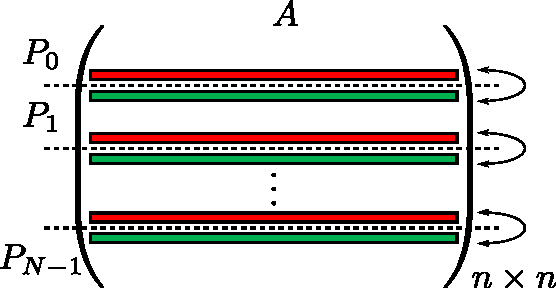
\includegraphics[width=0.45\textwidth]{images/a-matrix}
    \caption{Diagram of the partition of the matrix $A$}
    \label{fig:a-matrix}
\end{figure}

First of all, we need to define some variables in our C program that are needed for the MPI implementation, like \inline{rank}, \inline{size}, \inline{m}, \inline{ri}, \inline{rf}; and to initialize the MPI parallel region:

\begin{lstlisting}[firstnumber=52]
 // Variables needed for MPI
int rank, size;
\end{lstlisting}

We define the initial and final row of the subpartitions of the matrix as
\begin{align}
\begin{aligned}
    r_{i}[k] &= \frac{n}{N} \times \qty k \\
    r_{f}[k] &= \qty( \frac{n}{N} \times (k + 1) ) - 1 \\
\end{aligned}        
\end{align}
where $n$ is the dimension of the matrix, $N$ (or \inline{size}) is the amount of threads used, and $k = 0, \dots, N-1$ (or \inline{rank}) is the number of the working thread. Notice that Thread 0 will be used to make calculations as well as being the master thread to coordinate all computations. Notice that $n/N$ must be an integer.
 
\begin{lstlisting}[firstnumber=75]
// Initialisation of MPI parallel region
MPI_Init(&argc, &argv);
MPI_Comm_rank(MPI_COMM_WORLD, &rank);
MPI_Comm_size(MPI_COMM_WORLD, &size);
MPI_Status status;

// Define the partition of the matrix
int m = n/size;
int ri = rank * m, 
int rf = (rank+1) * m-1;
\end{lstlisting}

In the main loop of the program, we implement the basic parallel solution as described above. In the snippets below we can see excerpts of the script where MPI has been used. The rest of the program is almost identical to the standard implementation without MPI.

We can send and recieve messages from the different threads:
\begin{lstlisting}[firstnumber=96]
// Interchange of messages between consecutive rows
if ( rank > 0 ) {
	MPI_Send(&A[ri*n], n, MPI_FLOAT, rank-1, 1, MPI_COMM_WORLD);
	MPI_Recv(&A[(ri-1)*n], n, MPI_FLOAT, rank-1, 2, MPI_COMM_WORLD, &status);
}
if ( rank < size-1 ) {
	MPI_Send(&A[rf*n], n, MPI_FLOAT, rank+1, 2, MPI_COMM_WORLD);
	MPI_Recv(&A[(rf+1)*n], n, MPI_FLOAT, rank+1, 1, MPI_COMM_WORLD, &status);
}
\end{lstlisting}

The main part of the program, performing the Laplace step function using the implemented partition of the matrix $A$:
\begin{lstlisting}[firstnumber=106]
// Computation of the Laplace Step using MPI
if ( rank == 0 ) {
	for ( j = ri+1; j <= rf; j++ ) {
		for ( i = 1; i < n-1; i++ ) {
			temp[j*n+i] = stencil(A[j*n+i+1], A[j*n+i-1], A[(j-1)*n+i], A[(j+1)*n+i]);
			error = max_error( error, temp[j*n+i], A[j*n+i] );
		}
	}
}
if ( rank == (size-1) ) {
	for ( j = ri; j < rf; j++ ) {
		for ( i=1; i < n-1; i++ ) {
			temp[j*n+i] = stencil(A[j*n+i+1], A[j*n+i-1], A[(j-1)*n+i], A[(j+1)*n+i]);
			error = max_error( error, temp[j*n+i], A[j*n+i] );
		}
	}
}
if ( rank != 0 && rank != (size-1) ) {
	for ( j = ri; j <= rf; j++ ) {
		for ( i = 1; i < n-1; i++ ) {
			temp[j*n+i] = stencil(A[j*n+i+1], A[j*n+i-1], A[(j-1)*n+i], A[(j+1)*n+i]);
			error = max_error( error, temp[j*n+i], A[j*n+i] );
		}
	}
}
\end{lstlisting}

We send the partial errors of each thread to the master:
\begin{lstlisting}[firstnumber=132]
// Sending partial errors to the master and computing the maximum to find the global error
if ( rank != 0 ) {
		MPI_Send(&error, 1, MPI_FLOAT, 0, 3, MPI_COMM_WORLD);
} else {
	errors[0] =error;
	for (i = 1; i < size; i++ ) {
		MPI_Recv(&errors[i], 1, MPI_FLOAT, i, 3, MPI_COMM_WORLD, &status);
	}
}
global_error = maximum(errors, size);
\end{lstlisting}

The master calcualtes the global error using the partial errors previously sent:
\begin{lstlisting}[firstnumber=143]
// Sending back the resulting error
if ( rank == 0 ) {
	for(i = 1; i<size; i++ ) MPI_Send(&global_error, 1, MPI_FLOAT, i, 4, MPI_COMM_WORLD);
} else {
	MPI_Recv(&global_error, 1, MPI_FLOAT, 0, 4, MPI_COMM_WORLD, &status);
}
\end{lstlisting}

As usual, once we've finished the computations, we need to \emph{close} MPI.
\begin{lstlisting}[firstnumber=156]
MPI_Finalize();
\end{lstlisting}

As it can be seen, it is almost the same algorithm implemented in the provided \inline{lapFusion.c} code, just distributing the work and adding the data interchange among processes.
%-----------------------------------------------------------------
%	PERFORMANCE
%	!TEX root = ./../main.tex
%-----------------------------------------------------------------
\section{Assessment of the solution}\label{sec:assessment}

%-----------------------------------------------------------------
\subsection{Analysis with TAU}

Up to this point we are well aware of how the performance increases using OpenMP as a tool to parallelise the code. So now we want to explore further parallelisation, but using MPI this time. Once again we are going to use TAU, a toolkit for analysis performance that allows us to study in detail the performance of many parts of the code that we have parallelised.

As a comparison, we have used the same code as before with the same number of iterations and problem size.

%-----------------------------------------------------------------
\subsection{Influence of the number of threads}

%-----------------------------------------------------------------
\subsubsection{Using profile files (\texttt{paraprof})}

The toolkit \inline{paraprof} (bundled with TAU) allows us to parallel profile analysis. This is similar to using \inline{perf stat}, but now we have data for each of the threads.

For this part, we need to set the following environment variable:
\begin{lstlisting}
export TAU_PROFILE=1
\end{lstlisting}

Then we have to compile our source code using TAU, and then run it as usual
\begin{lstlisting}
tau_cc.sh -lm laplaceMPI.c -o mpiruntau
mpirun -np N ./mpiruntau 512 500
\end{lstlisting}
where \inline{N} can be 2 or 4.

This will give us \inline{profile.0.0.*} profile files; one for each of the threads used. To read and analyse these files we can use the \inline{paraprof} tool.

\bigskip

The result of the execution of the program using 2 and 4 threads can be seen in the tables \ref{tab:paraprof2}, \ref{tab:paraprof4} and figures \ref{fig:paraprof2-heat}, \ref{fig:paraprof4-heat} below. They show quite interesting results. On one hand we can see how the \emph{Run Time} of execution of the internal MPI operations are pretty much the same. The only main difference is the execution of the whole program itself; this is the calculation of the Laplace step.

An interesting conclusion that can be extracted from these graphs is that all threads are performing more or less the same. This is reflected in the fact we can not appreciate a big difference in the time needed for every thread; they all took the same time to finish the same work. This would be completely different if we have assigned a specific thread to act as a master only, instead of the master doing calculations as well.

\begin{table}[H]
    \centering
    \begin{tabular}{l c c}
        \toprule
        \toprule
        \textbf{Function} & \textbf{Thread 0}    & \textbf{Thread 1} \\
        \midrule
        \texttt{MPI\_Init()}       & \num{283}   & \num{282}   \\
        \texttt{MPI\_Comm\_size()} & \num{0}     & \num{0}     \\
        \texttt{MPI\_Comm\_rank()} & \num{0}     & \num{0.001} \\
        \texttt{MPI\_Send()}       & \num{0.877} & \num{1}     \\
        \texttt{MPI\_Recv()}       & \num{47}    & \num{50}    \\
        \texttt{MPI\_Finalize()}   & \num{81}    & \num{81}    \\
        \texttt{.TAU application}  & \num{7139}  & \num{7138}  \\
        \bottomrule
    \end{tabular}
    \caption{Run time (in ms) obtained on 2 threads}
    \label{tab:paraprof2}
\end{table}

\begin{figure}[H]
	\centering
	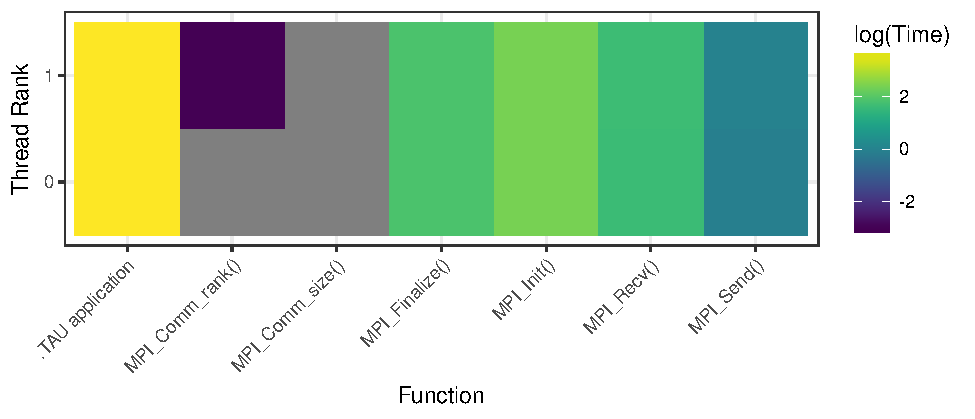
\includegraphics[width=0.95\textwidth]{images/pprof-2}
	\caption{Heatmap of the run time (in ms) obtained on 2 threads}
	\label{fig:paraprof2-heat}
\end{figure}

\begin{table}[H]
    \centering
    \begin{tabular}{l c c c c}
        \toprule
        \toprule
        \textbf{Function} & \textbf{Thread 0} & \textbf{Thread 1} & \textbf{Thread 2} & \textbf{Thread 3} \\
        \midrule
        \texttt{MPI\_Init()}       & \num{298}  & \num{284}  & \num{281}  & \num{276}  \\
        \texttt{MPI\_Comm\_size()} & \num{0}    & \num{0}    & \num{0}    & \num{0}    \\
        \texttt{MPI\_Comm\_rank()} & \num{0}    & \num{0}    & \num{0}    & \num{0}    \\
        \texttt{MPI\_Send()}       & \num{1}    & \num{1}    & \num{1}    & \num{1}    \\
        \texttt{MPI\_Recv()}       & \num{60}   & \num{28}   & \num{34}   & \num{55}   \\
        \texttt{MPI\_Finalize()}   & \num{81}   & \num{81}   & \num{82}   & \num{82}   \\
        \texttt{.TAU application}  & \num{3809} & \num{3795} & \num{3793} & \num{3788} \\
        \bottomrule
    \end{tabular}
    \caption{Run time (in ms) obtained on 4 threads}
    \label{tab:paraprof4}
\end{table}

\begin{figure}[H]
	\centering
	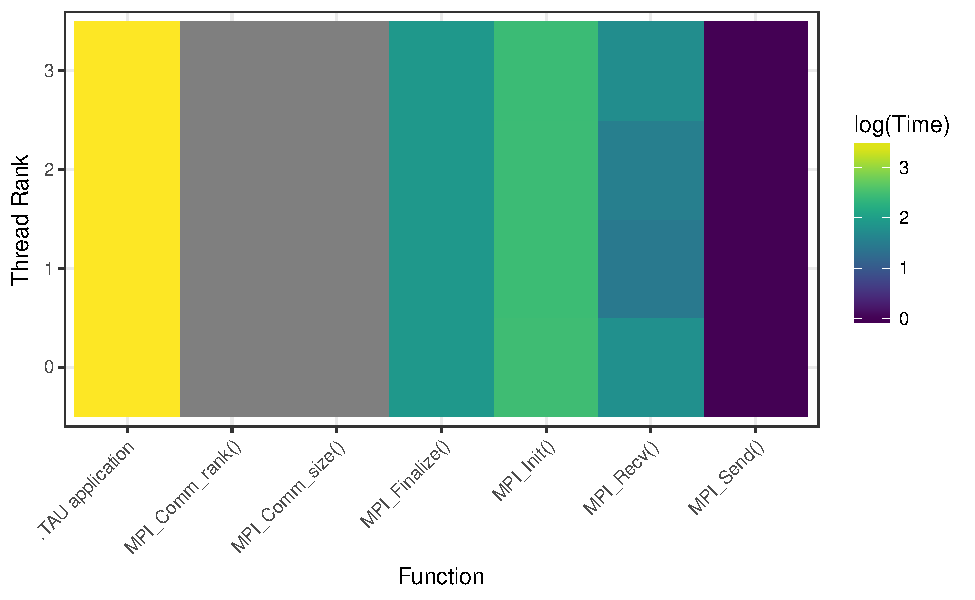
\includegraphics[width=0.95\textwidth]{images/pprof-4}
	\caption{Heatmap of the run time (in ms) obtained on 4 threads}
	\label{fig:paraprof4-heat}
\end{figure}

We can see that the time of this distributed version using MPI is $T/N + $ communication-overhead (where $T$ is the time it takes for the sequential algorithm to complete). Using 4 threads instead of 2 does not give us exactly half the compilation time; we get $\approx \SI{3800}{ms}$ instead of $\approx \SI{7100/2}{ms} = \SI{3550}{ms}$.

%-----------------------------------------------------------------
\subsubsection{Using traces (\texttt{jumpshot})}

Now that we have seen some of the standard measurement tools for parallelised code, we can explore even more detailed analytical tools. 

In particular, we aim to see the relations established between the threads and the information they process. This analysis could lead to a better insight on the strengths and weaknesses of our parallelisation and facilitate further improvement. 

In order to do so, we must first to arrange some technical issues.

First of all, we need to set the following environment variable:
\begin{lstlisting}
export TAU_TRACE=1
\end{lstlisting}

Then we have to compile our source code using TAU, and then run it as usual
\begin{lstlisting}
tau_cc.sh -lm laplaceMPI.c -o mpiruntau_trace
mpirun -np N ./mpiruntau_trace 512 500
\end{lstlisting}
where \inline{N} can be 2 or 4.

After doing this, we have to merge the obtained \inline{tautrace.0.0.*.trc} trace files into a readable \inline{.slog2} log file using the following commands:
\begin{lstlisting}
tau_treemerge.pl
tau2slog2 tau.trc tau.edf -o tauNthreads.slog2
\end{lstlisting}

To visualise the data of the logfile, we simply use the \inline{jumpshot} tool (also bundled with TAU):
\begin{lstlisting}
jumpshot tauNthreads.slog2
\end{lstlisting}

\bigskip

In figures \ref{fig:jumpshot2} and \ref{fig:jumpshot4} we can see an example of the Time Line of internal operations of each one of the used threads. Essentially, it shows us the information exchanged between different threads in chronological order. This helps us to understand how information/messages are sent and recieved by the different threads to perform the parallelisation. 

One crucial point of this visualisation is to spot redundancies or any kind of misperformance within the code.

\begin{figure}[H]
	\centering
	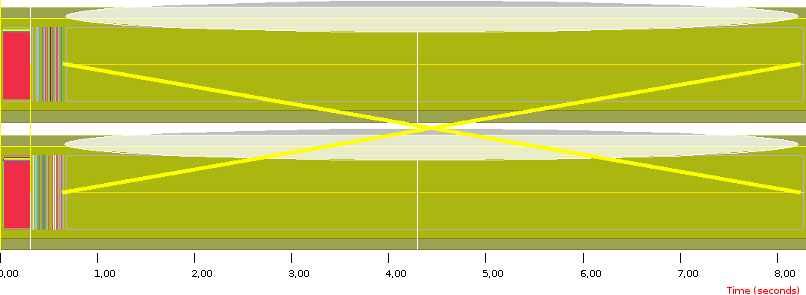
\includegraphics[width=0.85\textwidth]{images/trace2b}
	\caption{Time Line of the 2 threads using \inline{jumpshot}}
	\label{fig:jumpshot2}
\end{figure}

\begin{figure}[H]
	\centering
	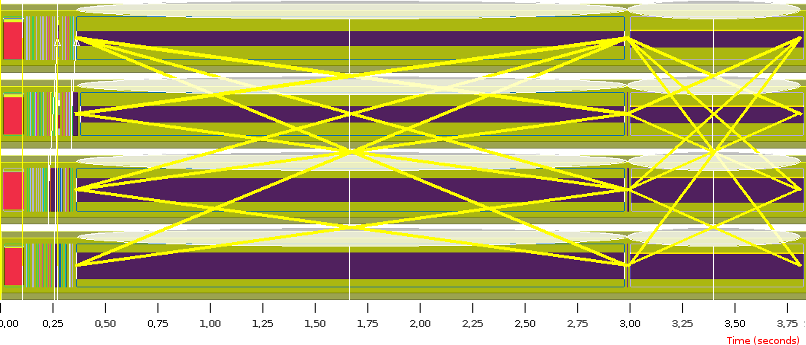
\includegraphics[width=0.85\textwidth]{images/trace4c}
	\caption{Time Line of the 4 threads using \inline{jumpshot}}
	\label{fig:jumpshot4}
\end{figure}

It is interesting to notice how the work is distributed and iteratively reorganised along the different threads within the timeline of the computation.

%-----------------------------------------------------------------
\subsection{Influence of the problem size}

%-----------------------------------------------------------------
\subsubsection{Using profile files (\texttt{paraprof})}

Up until now, we have learnt how our code behaves when different degrees of parallelisation are applied. Moreover, we now know some of the internal details involved in the performance of our new optimised code. 

One question that we now could ask ourselves is how the performance of the code scales. Until now we have studied the increase in the performance for a given magnitude of the matrix, but we have not considered how a change in this magnitude could affect the the computational effort needed to solve it. At first sight, we could guess that the larger the size of the matrix, the longer it will take to finish the problem. But, would all functions within the code increase in the same way? Or some functions would be more affected than others?

One way to address these questions and evaluate the scalability is simply to run the code for different matrix sizes and measure the time needed each time.

For this part, we need to set the following environment variables:
\begin{lstlisting}
export TAU_PROFILE=1
export TAU_TRACE=0
\end{lstlisting}

Then we have to compile our source code using TAU, and then run it as usual
\begin{lstlisting}
tau_cc.sh -lm laplaceMPI.c -o mpiruntau
mpirun -np 4 ./mpiruntau n 500
\end{lstlisting}
where we have chosen \inline{n} to be 128, 256, 384, 512, 640, and 768.

\begin{table}[H]
    \centering
    \resizebox{\textwidth}{!}{%
    \begin{tabular}{l c c c c c c}
        \toprule
        \toprule
        \textbf{Function} & $\mathbf{128 \times 128}$ & $\mathbf{256 \times 256}$ & $\mathbf{384 \times 384}$ & $\mathbf{512 \times 512}$ & $\mathbf{640 \times 640}$ & $\mathbf{768 \times 768}$ \\
        \midrule
        \texttt{MPI\_Init()}       & \num{287}     & \num{334}  & \num{284}     & \num{281}    & \num{280}     & \num{281}     \\
        \texttt{MPI\_Comm\_size()} & \num{0.0005}  & \num{0}    & \num{0.00025} & \num{0.0005} & \num{0.00075} & \num{0.0005}  \\
        \texttt{MPI\_Comm\_rank()} & \num{0.00025} & \num{0}    & \num{0}       & \num{0}      & \num{0.00025} & \num{0.00025} \\
        \texttt{MPI\_Send()}       & \num{0.583}   & \num{1}    & \num{1}       & \num{1}      & \num{1}       & \num{2}       \\
        \texttt{MPI\_Recv()}       & \num{7}       & \num{15}   & \num{12}      & \num{13}     & \num{13}      & \num{13}      \\
        \texttt{MPI\_Finalize()}   & \num{82}      & \num{282}  & \num{81}      & \num{82}     & \num{82}      & \num{119}     \\
        \texttt{.TAU application}  & \num{600}     & \num{1618} & \num{2299}    & \num{3781}   & \num{5483}    & \num{7705}    \\
        \bottomrule
    \end{tabular}}
    \caption{Run time (in ms) obtained on 4 threads for different problem sizes}
    \label{tab:paraprof-sizes}
\end{table}

\begin{figure}[H]
	\centering
	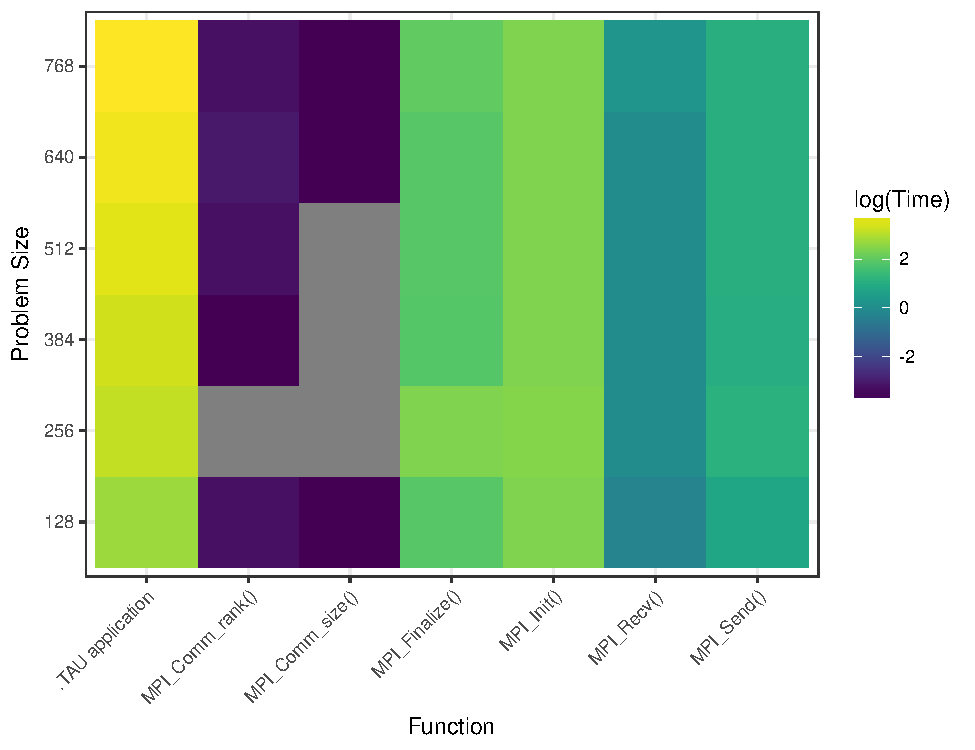
\includegraphics[width=0.95\textwidth]{images/pprof-sizes}
	\caption{Heatmap of the mean run time (in ms) obtained on 4 threads for different problem sizes}
	\label{fig:paraprof-sizes-heat}
\end{figure}

A possible concern involving the usage of MPI could be the loss of efficiency caused by the constant interchange of information between the threads. This loads more work to our code and thus can slow down the final output of the code, even though we aim to increase the performance thanks to making some processes parallel. We have checked that this not happens for a matrix where $n = 512$, because the improvement caused thanks to the parallelisation largely overcomes the possible lack of performance that more lines of orders could cause. Then, a still reasonable concern would be asking whether the parallelisation is also worth it for different dimensions of the problem. 

Table \ref{tab:paraprof-sizes} shows how the time needed to execute our program increases over the size of the problem. Looking at figure \ref{fig:paraprof-sizes-heat}, we can visualise and distinguish where this increase in time is happening; and notice that the function \inline{.TAU application} is the one suffering an increase in time execution, whereas all others increase are clearly negligible, if existent. That function is the one responsible for the computations of the matrix, whilst the others are those MPI functions needed to exchange information between the different threads.

Every possible drawback is, then, absolutely dwarfed by the increase in the performance caused by the parallelisation method that we have implemented. And this effect becomes even greater when we increase the size of the problem.

%-----------------------------------------------------------------
%	CONCLUSIONS
%	!TEX root = ./../main.tex
%-----------------------------------------------------------------
\section{Conclusions}

During the resolution of this exercise, we have had the opportunity to manually create a parallel code, in contrast with the one we had optimised in the OpenMP assignment, that was itself an improvement from the very first code of the course. This time we have used a different methodology to paralellise the code, we have learned to take advantage of the GPU of our system, whose usage has increased dramatically over the past few years.

All of this has let us comprehend the importance of parallel programming when aiming for high performance computation, for we have experienced an incremental increase of the performance in the code we have been improving.

One of the most important things learn in this assignment has been the fact that one should not use OpenACC as a magic formula for improving the execution time of the code; one has to be aware of how the machine is working and optimise the code to really take advantage of the hardware capabilities of the system.


% \begin{appendices}
% \include{./contents/A-code}
% \end{appendices}

%-----------------------------------------------------------------
%	BIBLIOGRAPHY
%-----------------------------------------------------------------


% \printbibliography[heading=bibintoc]
% \setcounter{secnumdepth}{0}
% \section{References}
% \printbibliography[title={Articles}, type=article, heading=subbibliography]
% \printbibliography[title={Books}, type=book, heading=subbibliography]
% \printbibliography[title={Websites}, type=online , heading=subbibliography]
% \printbibliography[title={Basic}, keyword=basic , heading=subbibliography]
% \printbibliography[title={Data Sets}, keyword=dataset , heading=subbibliography]
% \printbibliography[title={Licenses}, keyword=license , heading=subbibliography]

\end{document}
